\chapter{Requirements}
\label{requirements}

\section{Introduction}

Requirements Elicitation is an important step in the development of a software application. There are a number of techniques possible, such as "interviewing, protocol analysis, repertory grid, work groups" \parencite{davis2006effectiveness}. Structured interviews "appear to be one of the most effective elicitation techniques in a wide range of domains and situations" \parencite{davis2006effectiveness}. 

While the time constraints on this project did not allow for an in depth study of the requirements, or requirements process, the importance of requirements is not to be understated. (Put Franklin(?) quote here!)

\section{Methods for Requirements Elicitation}

In eliciting possible requirements for the site, there was a discussion with three club members with varying backgrounds and experience within the club.

\begin{table}[H]
\caption{Stakeholders for Requirements Elicitation}
\begin{center}
    \begin{tabular}{ | l | l | l | l | l| p{5cm} |}
    \hline
    Name & Age Bracket & Club Role & Club Membership & Work Background \\ \hline
	S1 & 35 - 45& Committee Member & 5 years & Senior Software Engineer \\ \hline
	S2 & 18 - 25 & New Member & 1 year & Graduate Software Engineer \\ \hline
	S3 & 55+ & Senior Member & 10+ years & Retired Public Servant \\ \hline
    \end{tabular}
\end{center}
\label{fig:userelicit}
\end{table}


\subsection{Storyboarding}

At an early stage of the application, rough storyboards were prepared for the FYP presentation. These storyboards were used to demonstrate how a page, such as the timetable shown in Figure~\ref{fig:timetableSB}, would be displayed by the application.

\begin{figure}[H]
\begin{center}
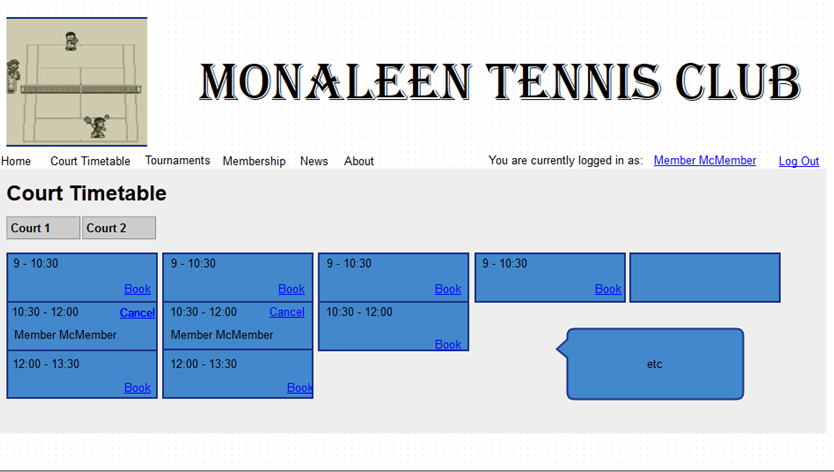
\includegraphics[width=14cm]{storyboard.png}
\end{center}
\caption{Timetable Storyboard, October 2013}
\label{fig:timetableSB}
\end{figure}

The storyboarding visualised aspects of the site, and gave a rough idea of functionality that would be needed within the application. These were shown to interviewees in order to help them visualise requirements.

\subsection{Exploratory Interviews}

In order to elicit requirements, a number of interviews were held with stakeholders. A set of questions were prepared as a guideline, and some storyboards were presented. The Tralee Tennis Club website was also presented to the interviewees.

\begin{enumerate}
\item Are you aware there is a site for Monaleen Tennis Club?
\item If are, what do you you it for?
\item What are the best features of the site? 
\item What features are needed?
\item If you were not aware, why? 
\item Would you use a website if you had known it was there?
\item Looking at the examples provided, are there any things you feel this club could benefit from?
\item How do you feel current tournaments are organised?
\item Is it easy to register for tournaments?
\item Have you ever had issues finding information about club events?
\item Do you know when club events are happening?
\item Is it easy to contact club members or find out how to contact them?
\item How easy is it to become a member/renew your membership?
\item How do you contact club committee members?  
\end{enumerate}


During the elicitation process a number of areas were highlight as desired features.

\begin{enumerate}
\item Online Timetable
\begin{itemize}
\item Allow members to view courts and make/view bookings
\end{itemize}
\item Tournaments
\begin{itemize}
\item Allow user to register for a tournament, and view tournaments ongoing.
\end{itemize}
\item Contact Members
\begin{itemize}
\item Easy way to contact all members
\end{itemize}
\item Member Directory
\begin{itemize}
\item A list of all members, contact details, roles
\end{itemize}
\item News Section
\begin{itemize}
\item Create new items to display for members
\end{itemize}
\item Members Area
\begin{itemize}
\item A secure area that only members could access
\end{itemize}
\item Member Application
\begin{itemize}
\item Automated registration, replace old paper form
\end{itemize}
\item Club Map
\begin{itemize}
\item Directions to the club for new members and non-local visitors
\end{itemize}
\item Contact Details
\begin{itemize}
\item Information on how to contact within the club for specific needs
\end{itemize}
\item Statistics
\begin{itemize}
\item Such as games played, Win/Loss ratio
\end{itemize}
\end{enumerate}
\begin{table}[H]
\label{fig:requirementsFeatures}
\caption{Requested Features}
\end{table}
Table ~\ref{fig:reqbreakdown} refers to each numbered requirement, and whether it was brought up by a stakeholder during the elicitation process.
\begin{table}[H]
\caption{Requested Feature Breakdown}
\begin{center}
    \begin{tabular}{ | l | l | l | l| l| l| l| l| l|l| p{.22cm} |}
    \hline
     \textit{Name}& 1& 2 & 3 & 4 & 5 & 6 & 7 & 8 & 9 & 10\\ \hline
	 S1 & N & Y & Y & Y & Y & Y & Y & Y & Y & N\\ \hline
	 S2 & Y & Y & Y & N & N & N & N & N & N & Y\\ \hline
	 S3 & Y & N & N & N & N & N & Y & Y & N & N\\ \hline
  Total & 2 & 2 & 2 & 1 & 1 & 1 & 2 & 2 & 1 & 1\\ \hline
    \end{tabular}
\end{center}
\label{fig:reqbreakdown}
\end{table}

\section{Focus group}

With the information obtained from the exploratory interviews, a focus was held with the interviewees in order to obtain more detail on what functional requirements would be needed to implement any site features. These features were broken down into four categories: \textit{Timetable}, \textit{Tournaments}, \textit{Members}, and \textit{News}.

\section{Functional Requirements}

\subsection{Timetable} 

The timetable is the core aspect of the application, and one that would be most likely to be used by all members, not just those involved competitively. While the regular member would only be concerned with the booking of slots, there are a number of requirements defined for use by the administrator in order to configure a relevant timetable not the club. The timetable needs to be flexible to allow the administrator full control at all stages.

\begin{enumerate}
\item Flexible 
\item Edit individual slots
\item Define a template for a timetable
\item Reset timetable
\item Define look ahead for timetable (how many weeks in advance a user can see)
\item Delete timetable
\item Enable and disable timetable
\item Timetable analysis (No slots free, booked etc)
\end{enumerate}

\subsection{Tournament}

The tournament is a section that would be heavily used by those players who compete regularly. Key requirements for all users were the ability to view, and register for, tournaments. Administrators would need to be able to create and control tournaments within the application.

\begin{enumerate}
\item Create tournament
\item Delete tournament
\item Enable user signup
\item Finalize user signup
\item Display tournament times
\item Create different kinds of tournaments
\item Organise members into teams
\item Contact all members in tournament
\item Statistics
\end{enumerate}


\subsection{News}

The news section is the main contact point between the committee and members of the club. All committee members should have access to the ability to create, and delete, news. 

\begin{enumerate}
\item Create news
\item Delete news
\item Allow more than one person to post news
\end{enumerate}

\subsection{Members}

A key finding was a easy to use registration system, as the current paper based system can be problematic as it is necessary to contact one person to become a club member. Administration management of existing and potential members was also an area that was highlighted as key to any system.

\begin{enumerate}
\item Member registration
\item Member only access
\item Approve/Block members
\item Edit profiles
\item View all Members
\item Contact Members
\end{enumerate}

\section{Non Functional Requirements}

As a software developer, S1 mentioned a number of areas that would also need to be part of the application. These attributes were key to having the application being useful to both the club and its members.

\subsection{Security}

Since user details would be stored in the application, security of this data was highlighted as a concern. While no payment information would be held by the application, there would be names, addresses and phones numbers held within the application. The security of this information would need to be ensured.

\subsection{Extensibility}

Extensibility of the application was discussed with particular attention of the ability of the application to deal with changed to the club structure. Currently, the club has two courts in which users can book time for games. It is likely that the club will be expanding in the near future. This will result in the creation of four next courts in the near future. The application should be able to scale with this possibility without issue.

Tournaments were also mentioned as an area where future requirements may stem from. Currently, the club operates three kinds of tournaments: Singles, Doubles and Mixed Doubles. These are broken down into Ladder style tournaments and Bracket style tournaments. The club regularly holds tournaments with other national tennis clubs. The ability to create tournaments that suit these events could be necessary.

\subsection{Usability}

The age of the club members range from 8 to 80, so ease of use of any software solution is important. If a system is going to replace the existing system that all can use, a similar level of usability is required. The most common function used by members is the reservation of time slot in one of the courts. A software alternative needs to be intuitive for all members.

\subsection{Performance}

The site needs to be fast to use, and cheap to run. There's no funds to pay for a high end server, so it needs to be able to run on a virtual server, or a Amazon micro-instance, without any performance hits. It also needs to be able to cope with multiple users at the same time. 

\section{Use Cases}

\begin{usecase}
\addtitle{Use Case 1}{View All Members} 
\addfield{Scope:}{System-wide}
\addfield{Level:}{User can view a list of all registered, and approved, members of the club}
\addfield{Primary Actor:}{All Registered and Authenticated Users}
\additemizedfield{Stakeholders and Interests:}{
	\item All Users: contact information for club members
}

\addfield{Preconditions:}{User is registered and approved}
\addfield{Postconditions:}{User must be authenticated by the framework}
\addscenario{Main Success Scenario:}{
	\item User logs in
	\item User clicks on View Members
	\item System displays member information
}
\addscenario{Extensions:}{
	\item[1.a] Invalid login data:
		\begin{enumerate}
		\item[1.] System shows failure message
		\item[2.] User returns to step 1
		\end{enumerate}
	\item[1.a] User not approved:
		\begin{enumerate}
		\item[1.] System shows failure message
		\item[2.] Admin is emailed about attempted access by unapproved member
		\end{enumerate}
}
\addfield{Frequency of Occurrence:}{High}
\end{usecase}

\section{Conclusion}

The interview process, in collaboration with storyboarding, gave a wide range of potential requirements to be implemented in the final application. It also showed demand for certain features, and allowed requirements to be prioritised to meet this demand.